\documentclass{article}
\usepackage[utf8]{inputenc}
\usepackage[english]{babel}
\usepackage{amsmath}
\usepackage{ulem}
\usepackage{verbatim}
\usepackage{graphicx}
\usepackage{palatino}
\linespread{1.05}
\title{}
\author{Ronni Elken Lindsgaard}
\begin{document}
\maketitle
\section{Serializability \& Locking}
The predecence graph for Schedule 1 can be seen in figure \ref{fig:schedule1}.
As there is a cycle the schedule is not conflict-serializable. The schedule
could not have been generated using strict two-phase locking as the write to X
in T2 needs to happen after the read in T1. T1 cannot be completed and thus
releasing the lock of X as T3 needs to release the read lock for Y. T3 cannot
run before T2 which is visible in the predence graph. 

\begin{figure}[H]
  \centering
  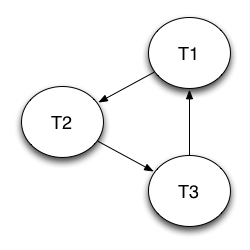
\includegraphics[width=0.5\textwidth]{images/schedule1}
  \caption{Precedence graph for Schedule 1. The cycle shows that the schedule is
  not conflict-serializable.}
  \label{fig:schedule1}
\end{figure}


Figure \ref{fig:schedule2} show the precedence graph for Schedule 2. There is no
cycle which means it is conflict serializable. Figure \ref{fig:schedule2-2pl}
shows injected read/write locks in accordance with strict 2PL rules.
 
\begin{figure}[H]
  \centering
  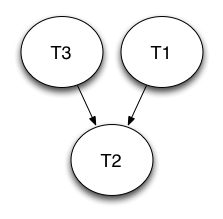
\includegraphics[width=0.5\textwidth]{images/schedule2}
  \footnotesize
  \caption{Precedence graph for Schedule 2. The absence of a cycle show that the
  schedule is conflict-serializable.}
  \label{fig:schedule2}
\end{figure}

\begin{figure}[H]
\footnotesize
\centering
\verbatiminput{figures/schedule2-2pl.txt}
\caption{Schedule 2 with read- (RL) and writelocks (WL) induced. All locks are
released on commits. The unlock operations are omitted for simplicity of the
table.}
\label{fig:schedule2-2pl}
\end{figure}

\end{document}

